\documentclass{article}
\usepackage{pdfpages}
\usepackage{graphicx}  % For PNG
\usepackage[left=2cm, right=2cm, top=2cm]{geometry}

% Give Table of Contents Hyperlinks
\usepackage{hyperref}
\hypersetup{
    colorlinks,
    citecolor=black,
    filecolor=black,
    linkcolor=black,
    urlcolor=blue
}
\pagenumbering{gobble}
% \pagenumbering{roman} % set the numbering style to lowercase letter

\title{\textbf{Homework 3}}

\author{MacMillan, Kyle}
\date{October 12, 2018}

\begin{document}


\addcontentsline{toc}{section}{Title}
\maketitle

\newpage
\tableofcontents
\addcontentsline{toc}{section}{Table of Contents}

\pagenumbering{roman}   % Set TOC page numbering to lowercase roman numerals



%%%%%%%%%%%%%%%%%%%%%%%%%%%% INTRO SECTION %%%%%%%%%%%%%%%%%%%%%%%%%%%%
\newpage
\hypersetup{
    colorlinks,
    citecolor=blue,
    filecolor=black,
    linkcolor=blue,
    urlcolor=blue
}
\pagenumbering{arabic}  % Set content page numbering to arabic numerals

\setcounter{page}{1}
\newpage
\section{\textbf{Problem 6.5}}
Figure \ref{fig:6.5.a} shows the required plot.

\begin{figure}[h]
    \centering
    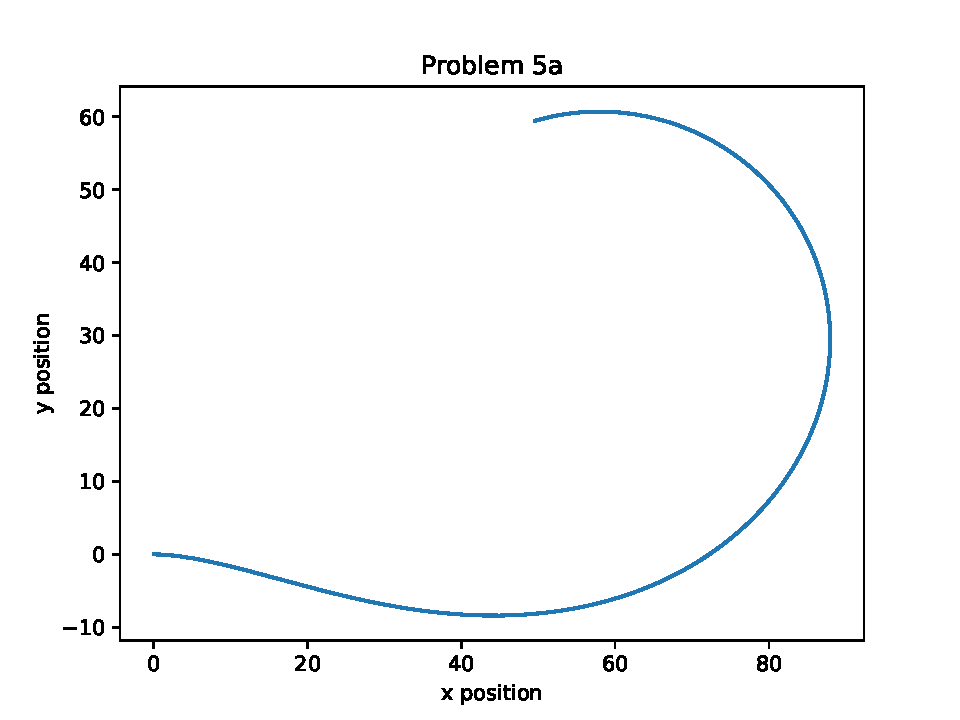
\includegraphics[pages=1]{p6-5-a}
    \caption{Problem 6.5.a}
    \label{fig:6.5.a}
\end{figure}


\newpage
\noindent Figure \ref{fig:6.5.b} shows the data points that were saved.

\begin{figure}[h]
    \centering
    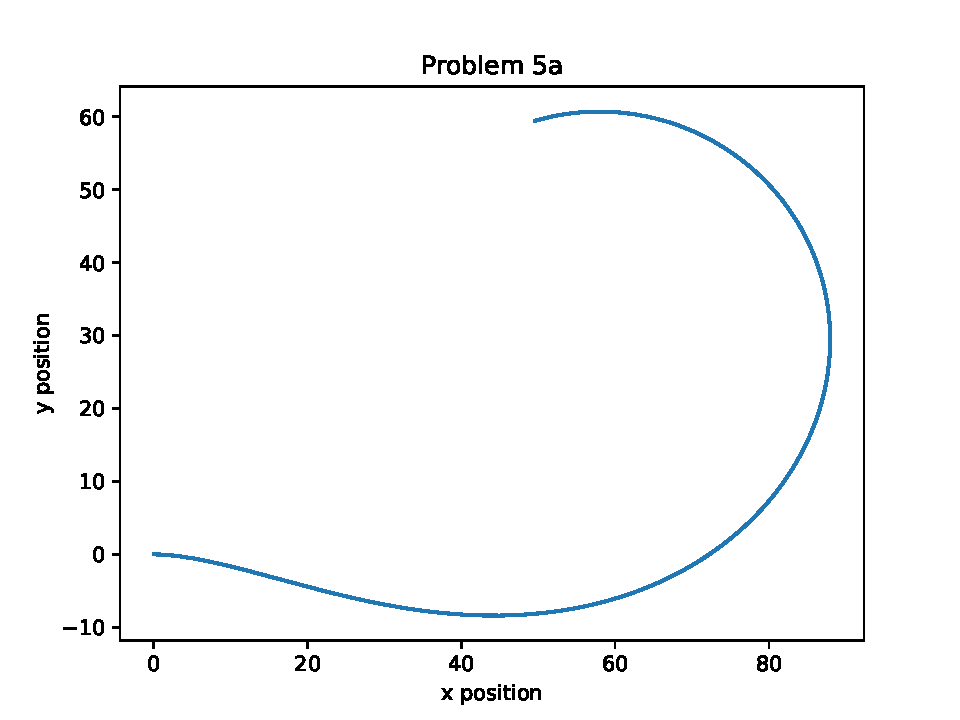
\includegraphics[pages=1]{p6-5-b}
    \caption{Problem 6.5.b}
    \label{fig:6.5.b}
\end{figure}


\newpage
Figure \ref{fig:6.5.c} shows the data points that were saved.

\begin{figure}[h]
    \centering
    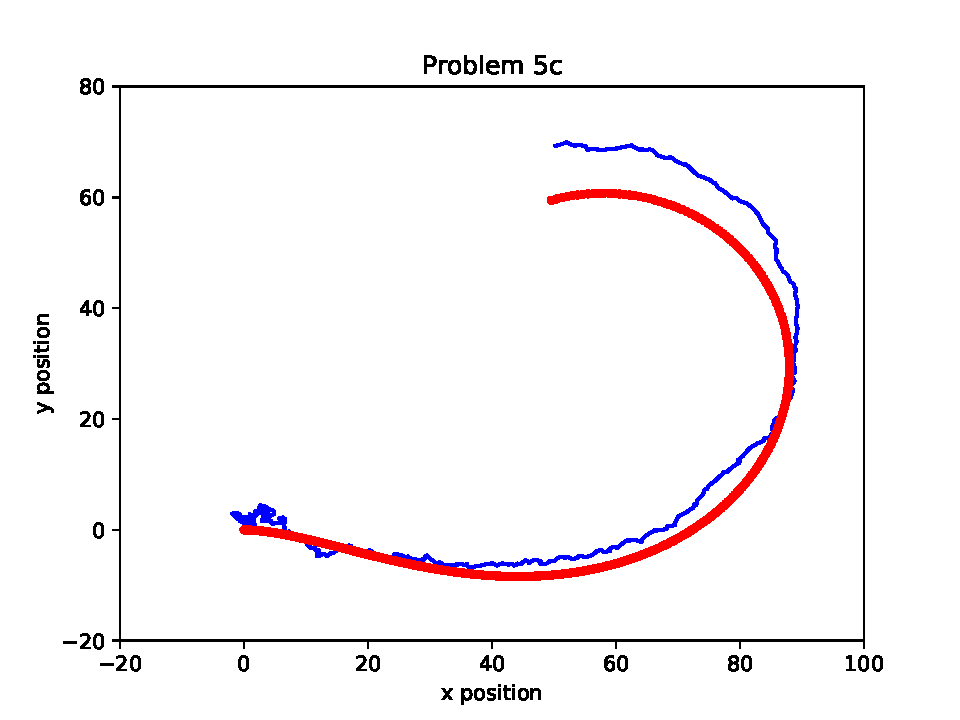
\includegraphics[pages=1]{p6-5-c}
    \caption{Problem 6.5.c}
    \label{fig:6.5.c}
\end{figure}


\newpage
Figure \ref{fig:6.5.d} shows the data points that were saved.

\begin{figure}[h]
    \centering
    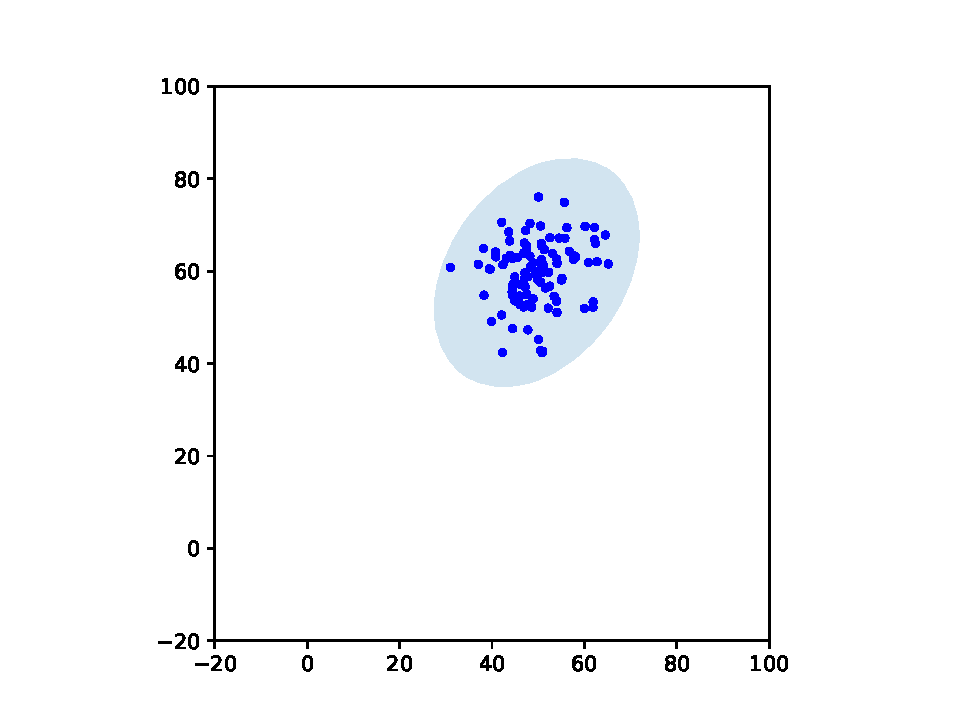
\includegraphics[pages=1]{p6-5-d}
    \caption{Problem 6.5.d}
    \label{fig:6.5.d}
\end{figure}


\newpage
\section{\textbf{Problem 6.8}}
For this problem we have to take into account $x$, $y$, and $\theta$ derivatives with respect to time for the parametric form of an ellipse. We also make the assumption that velocity is constant. Parametric forms of $x$, $y$, and $\theta$ are as follows:

$$x(t) = 3 + 4cos(t)$$

$$y(t) = 2 + 3sin(t)$$

$$\theta(t) = \pi + \phi(t)$$

The derivatives are as follows:

$$\hat{x}(t) = -4sin(t)$$

$$\hat{y}(t) = 3cos(t)$$

$$\hat{\theta}(t) = \frac{12sec^2(t)}{9tan^2(t) + 16}$$

The only reason $\hat{\theta}(t)$ is differentiable without chaos is because as the robot moves around, the angle is independent of the starting $x$ and $y$ position, so the equation used to calculate $\hat{\theta}(t)$ are as follows:

$$\theta(t) = \pi + arctan\Big(\frac{3sin(t)}{4cos(t)}\Big)$$

You then plug and chug those into the \href{http://roboscience.org/book/html/Motion/DriveSystems.html#equation-meccanuminversekinematics}{inverse kinematic equations} to get wheel speed of each wheel at every time step.



\end{document}
